\subsection{Notion}
paragraph{Basics}
\subparagraph{MultiVariate Normal}
Recall that the probability density functon for a \emph{MultiVariate Normal} in $D$ 
dimensions is
\begin{center}
    $\mathcal{N}(\bm{x}|\bm{\mu},\bm{\Sigma}) \triangleq 
    \dfrac{1}{(2\pi)^{\frac{D}{2}}|\Sigma|^\frac{1}{2}}
    e^{-\frac{1}{2}(\bm{x}-\mu)^{T}\Sigma^{-1}(\bm{x}-\bm{\mu})}$
\end{center}

\subparagraph{Mahalanobis}
corresponds to $-\dfrac{1}{2}(\bm{x}-\mu)^{T}\Sigma^{-1}(\bm{x}-\bm{\mu})$, which is 
the \emph{distance between} $\bm{x}$ \emph{and the mean vector} $\bm{\mu}$.\\
Let look at the \emph{eigendecomposition} of $\bm{\Sigma}$, then\\
$\bm{\Sigma} = \bm{U\Lambda U^{T}}$, with $\bm{U}$ is an orthonormal matrix satisfying 
$\bm{UU^{T}} = \bm{I}$ and $\bm{\Lambda}$ a
diagonal matrix of eigenvalues.
\begin{align*}
    \Sigma^{-1} &= U^{-T}\bm{\Lambda}^{-1}U^{-1}\\
                &= \bm{U}\bm{\Lambda}^{-1}\bm{U}^{T}\\
                &= \su{i=1}{D}\frac{1}{\lambda_{j}}\bm{u}\bm{u}_{j}^{T}
\end{align*}
where $\bm{u}_{j}$ is the $j$th eigenvector.\\
We can then write:
\begin{align*}
    (\bm{x}-\bm{u})^{T}\Sigma^{-1}(\bm{x}-\bm{u}) &= 
        (\bm{x}-\bm{u})^{T}\su{i=1}{D}\frac{1}{\lambda_{j}}\bm{u}\bm{u}_{j}^{T}
        (\bm{x}-\bm{u})\\
                                                  &=
    \su{i=1}{D}\frac{1}{\lambda_{j}}(\bm{x}-\bm{u})^{T}\bm{u}\bm{u}_{j}^{T}(\bm{x}-\bm{u})
    \\
                                                  &= 
    \su{i=1}{D}\frac{y_{i}^{2}}{\lambda_{j}}
\end{align*}
Then for $D=2$ we have the equation of an ellipse. 
\begin{figure}[H]
    \begin{center}
        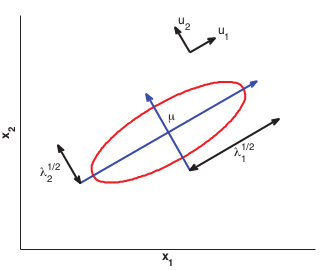
\includegraphics[width=\textwidth]{./chaps/32_sec/images/1_mahalanobis.png}
    \end{center}
    \caption{Mahalanobis distance interpretation in 2D}
    \label{fig:1_mahalanobis}
\end{figure}

\paragraph{MLE for an MVN}
\subparagraph{MLE for a Gaussian}
If we have $n$ samples $\bm{x}_{i} \hookrightarrow \mathcal{N}(\bm{\mu, \bm{\Sigma}})$\\
$\begin{cases}
    \hat{\bm{\mu}}_{mle} = \dfrac{1}{n}\su{i=1}{n}\bm{x}_{i} \triangleq 
    \overline{\bm{x}} \\
    \hat{\bm{\Sigma}}_{mle} = \dfrac{1}{n}\su{i=1}{n}(x_{i}-\overline{x})
    (\bm{x}_{i}-\overline{\bm{x}})^{T} = \dfrac{1}{N}\su{i=1}{n}
    \bm{x}_{i}\bm{x}_{i}^{T} - \overline{\bm{x}}\overline{\bm{x}}^{T}
\end{cases}$
That is, the \emph{MLE} is just the empirical mean and empirical covariance.
\subparagraph{Proof}
Reall that for $(\bm{a}, \bm{b}, \bm{A}, \bm{B}) \in \mathbb{R}^{n} \times \mathbb{R}^{n}
\times \mathcal{M}(\mathbb{R})_{n,n} \times \mathcal{M}(\mathbb{R})_{n,n}$ \\
$\begin{cases}
    \frac{\partial(\bm{b}^{T}\bm{a})}{\partial\bm{a}} = \bm{b}\\
    \frac{\partial(\bm{a}^{T}\bm{Aa})}{\partial\bm{a}} = (\bm{A} + \bm{A}^{T})\bm{a}\\
    \frac{\partial tr(\bm{AB})}{\partial\bm{a}} = \bm{B}^{T}\\
    \frac{\partial \log(|\bm{A}|)}{\partial\bm{A}} = \bm{A}^{-T} \triangleq 
    (\bm{A}^{-1})^{T}\\
    tr(\bm{ABC}) = tr(\bm{CAB}) = tr(\bm{BCA})\\
    \bm{x}^{T}\bm{A}\bm{x} = tr(\bm{xx}^{T}\bm{A}) = tr(\bm{Axx}^{T})
\end{cases}$\\
Then, with $\bm{\Lambda} = \bm{\Sigma}^{-1}$, log-likelihood is
\begin{align*}
    \dfrac{\partial l(\bm{\mu}, \bm{\Sigma})}{\partial\bm{\mu}} 
    &= \dfrac{\partial}{\partial\mu}\left(\dfrac{N\log(|\bm{\Lambda}|)}{2} - \dfrac{1}{2}
    \su{i=1}{n}(\bm{x}_{i} - \bm{\mu})^{T}\Lambda(\bm{x}_{i} - \bm{\mu})\right) \\
    &= -\dfrac{\partial \su{i=1}{n}(\bm{x}_{i} - \bm{\mu})^{T}\Sigma^{-1}(\bm{x}_{i}-
    \bm{\mu})}{2\partial\mu}\\
    &= -\su{i=1}{n}\dfrac{\partial (\bm{x}_{i} - \bm{\mu})^{T}\Sigma^{-1}(\bm{x}_{i}-
    \bm{\mu})}{2\partial\mu}\\
    &= -\su{i=1}{n}\dfrac{\partial \bm{x}_{i}^{T}\Sigma^{-1} - \bm{\mu}^{T}\Sigma^{-1}
        (\bm{x}_{i}- \bm{\mu})}{2\partial\mu}\\
    &= -\su{i=1}{n}\dfrac{\partial \bm{x}_{i}^{T}\Sigma^{-1}(\bm{x}_{i}- \bm{\mu}) - 
        \bm{\mu}^{T}\Sigma^{-1}(\bm{x}_{i}- \bm{\mu})
        (\bm{x}_{i}- \bm{\mu})}{2\partial\mu}\\
    &= -\su{i=1}{n}\dfrac{\partial \bm{x}_{i}^{T}\Sigma^{-1}\bm{x}_{i}- 
        \bm{x}_{i}^{T}\Sigma^{-1}\bm{\mu} - 
        \bm{\mu}^{T}\Sigma^{-1}\bm{x}_{i} + \bm{\mu}^{T}\Sigma^{-1}\bm{\mu}}
        {2\partial\mu}\\
    &= -\dfrac{1}{2}\su{i=1}{n} 0 - \dfrac{\partial \bm{x}_{i}}{\partial\bm{\mu}}
    \bm{\Sigma}^{-1}
    \bm{\mu} - \dfrac{\partial \bm{\mu}}{\partial\bm{\mu}}\bm{\Sigma}^{-T} \bm{x}_{i}
    - \dfrac{\partial \bm{\mu}}{\partial\bm{\mu}}\bm{\Sigma}^{-1}
    \bm{x}_{i} - \dfrac{\partial \bm{x}_{i}}{\partial\bm{\mu}}\bm{\Sigma}^{-T} \bm{\mu}
    + \dfrac{\partial \bm{\mu}^{T}\Sigma^{-1}\bm{\mu}}{\partial \bm{\mu}}\\
    &= -\dfrac{1}{2}\su{i=1}{n} - (\bm{\Sigma}^{-1}+\bm{\Sigma}^{-T})\bm{x}_{i} 
    + (\bm{\Sigma}^{-1}+\bm{\Sigma}^{-T})\bm{\mu}\\
    &= \dfrac{1}{2}\su{i=1}{n}(\bm{\Sigma}^{-1}+\bm{\Sigma}^{-T})(\bm{x}_{i}-\bm{\mu})\\
    &= \dfrac{1}{2}\su{i=1}{n}(\bm{\Sigma}^{-1}+\bm{\Sigma}^{-T})\bm{y}_{i}\\
    &= \bm{\Sigma}^{-1}\su{i=1}{n}\bm{y}_{i}\\
    &= 0_{p,p}
\end{align*}
Considering that $S_{\bm{\mu}} \triangleq \su{i=1}{n}(\bm{x}_{i} - \bm{\mu})
(\bm{x}_{i} - \bm{\mu})^{T}$
\begin{align*}
    \dfrac{\partial l(\Lambda)}{\partial\Lambda} 
    &= \dfrac{\partial}{\partial\Lambda}\left( \dfrac{n}{2}\log(|\Lambda|) -
        \dfrac{1}{2}\su{i=1}{n}tr\left([\bm{x}_{i}-\bm{\mu}]
    [\bm{x}_{i}-\bm{\mu}]^{T}\bm{\Lambda}\right)\right)\\
    &= \dfrac{\partial}{\partial\Lambda}\left(\dfrac{n}{2}\log(|\Lambda|) -
        \dfrac{1}{2}tr(\bm{S}_{\bm{\mu}}\bm{\Lambda})\right)\\
    &= \dfrac{1}{2}\left(n\Lambda^{-T} - \bm{S}_{\bm{\mu}}^{T}\right)\\
    &= 0_{p,p}
\end{align*}

\paragraph{Maximum entropy derivation of the Gaussian}
The multivariate Gaussian is the distribution with the maximum entropy subject to having
a specified mean and covariance. This is one reason the Gaussian is so widely used: the
first two moments are usually all that we can reliably estimate from the data, so we want
a distribution that captures these properties, but otherwise makes as few additional 
assumptions as possible.\\

\subparagraph{Theorem}
Let $q(x)$ be any density satisfying $\Su{}{}q(x)x_{i}x_{j} = \su{ij}{}$. Let 
$p = \mathcal{N}(0, \bm{\Sigma})$, then $h(q)\leq h(p)$

\subparagraph{Proof}
\begin{align*}
    0 &\leq \mathbb{KL}(q||p)\\
      &= \Su{}{}q(x)\log\left(\frac{q(x)}{p(x)}\right)dx
      &= \Su{}{}q(x)\log(q(x))dx - \Su{}{}q(x)\log(p(x))dx\\
      &= -h(q) - \Su{}{}q(x)\log(p(x))dx\\
      &= -h(q) - \Su{}{}p(x)\log(p(x))dx\\
      &= -h(q) + h(q)
\end{align*}
The 2nd line from the bottom follows since $q$ and $p$ yield the same moments for the 
quadratic form encoded by $\log(p(x))$






